\section{Medições em laboratório}

Nesta seção, são apresentados os detalhes e resultados das medições realizadas no experimento, com o objetivo de obter dados quantitativos para análise e validação dos resultados teóricos previamente obtidos.

\begin{figure}[H]
    \centering
    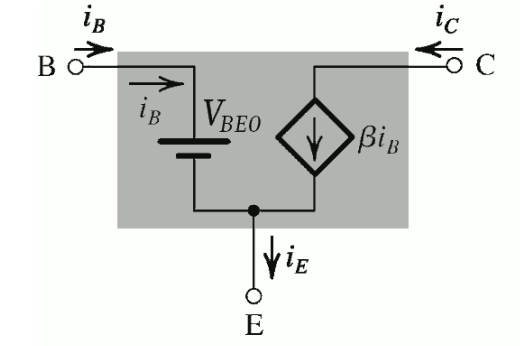
\includegraphics[width=0.5\columnwidth]{images/modelo_grandes_sinais.png}
    \caption{Circuito montado em laboratório.}
\end{figure}

\subsection{Componentes}

Os seguintes valores foram medidos para os componentes que foram empregados no circuito:

\begin{equation}
    \begin{aligned}
         & R_1 = 11743           \\
         & R_2 = 2650            \\
         & R_c = 470             \\
         & R_e = 178.4           \\
         & R_L = 145.5           \\
         & C_1 = 10.245 \mu F    \\
         & C_2 = 107.25 \mu F    \\
         & C_3 = 106 \mu F       \\
         & Potenciometro = 10.3k
    \end{aligned}
\end{equation}

\subsection{Medições de grandes sinais}

Para grandes sinais considera-se que os capacitores estao em aberto. Logo, na pratica isto implica em remover os capacitores do circuito e realizar as medicoes. Os resultados obtidos estao apresentados a seguir:

\begin{equation}
    \begin{aligned}
         & V_{cc} = 8.006  V \\
         & V_{ee} = -8.006 V \\
         & V_b = - 5.12 V    \\
         & V_e = -5.7 V      \\
         & V_c = 2.14 V      \\
         & V_{rc} = 5.87 V   \\
    \end{aligned}
\end{equation}

\subsection{Medições de pequenos sinais}

No contexto de pequenos sinais, é comum considerar que os capacitores atuam como componentes de baixa impedância, funcionando praticamente como curtos-circuitos. Portanto, na aplicação prática, essa premissa implica na inclusão dos capacitores no circuito para, em seguida, efetuarmos as medições necessárias. Nossa configuração envolve uma tensão de entrada, denotada por $V_i$, com uma amplitude de $50 mV_{pp}$ e frequência de $10 kHz$.

\subsubsection{$V_{be}$}

\begin{figure}[H]
    \centering
    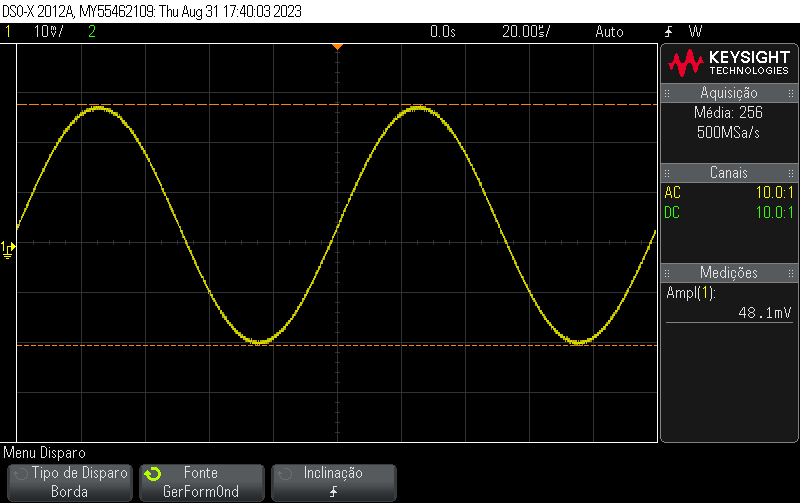
\includegraphics[width=0.5\columnwidth]{images/v_be.png}
    \caption{Tensão sobre $V_{be}$.}
\end{figure}

\subsubsection{$V_{o}$}

\begin{figure}[H]
    \centering
    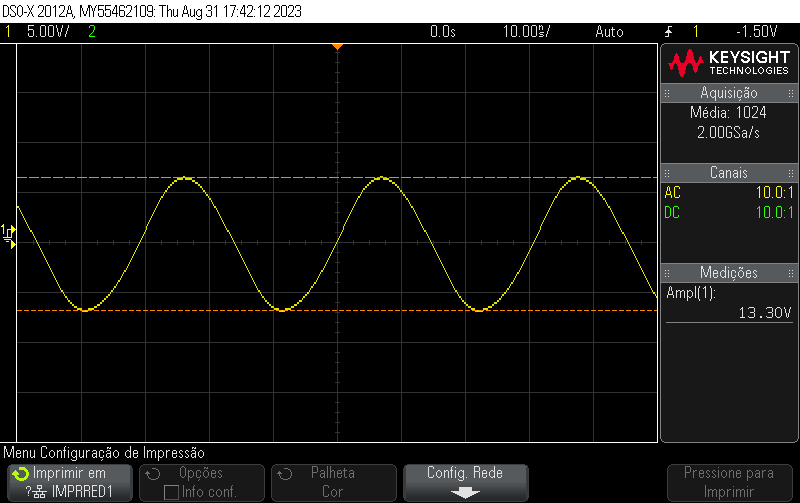
\includegraphics[width=0.5\columnwidth]{images/V_o.png}
    \caption{Tensão sobre $V_{o}$.}
\end{figure}

\subsubsection{$V_{o}$}

\begin{figure}[H]
    \centering
    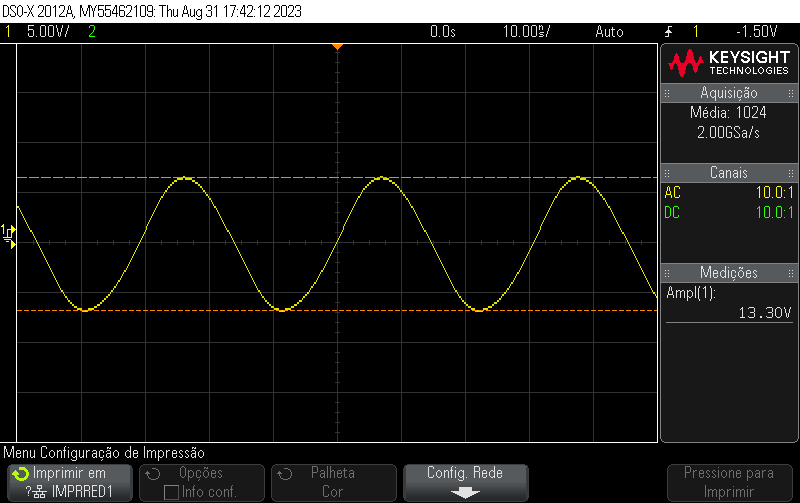
\includegraphics[width=0.5\columnwidth]{images/V_o.png}
    \caption{Tensão sobre $V_{o}$.}
\end{figure}


\subsubsection{$V_{L}$}

\begin{figure}[H]
    \centering
    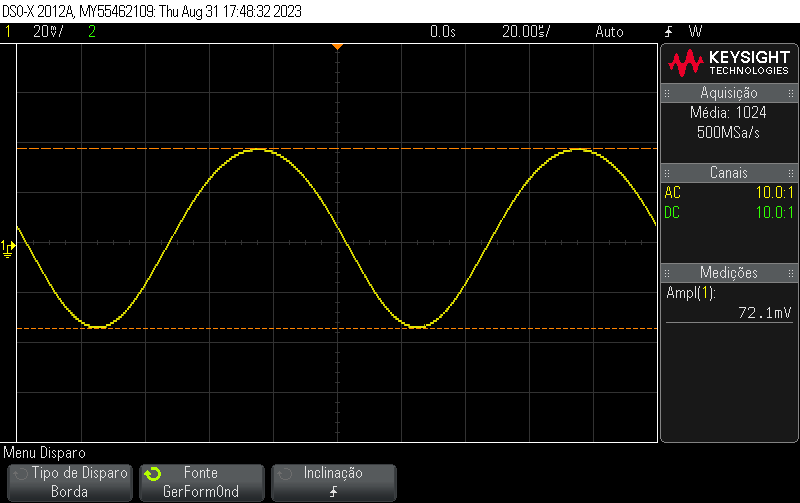
\includegraphics[width=0.5\columnwidth]{images/V_L.png}
    \caption{Tensão sobre $V_{L}$.}
\end{figure}

\subsubsection{Tensões sobre potenciometro e $R_L$}

Aqui mede-se cinco pontos de tensão sobre o potenciômetro e $R_L$ para diferentes valores de resistência do potenciômetro. Os resultados obtidos estão apresentados a seguir:

\begin{figure}[H]
    \centering
    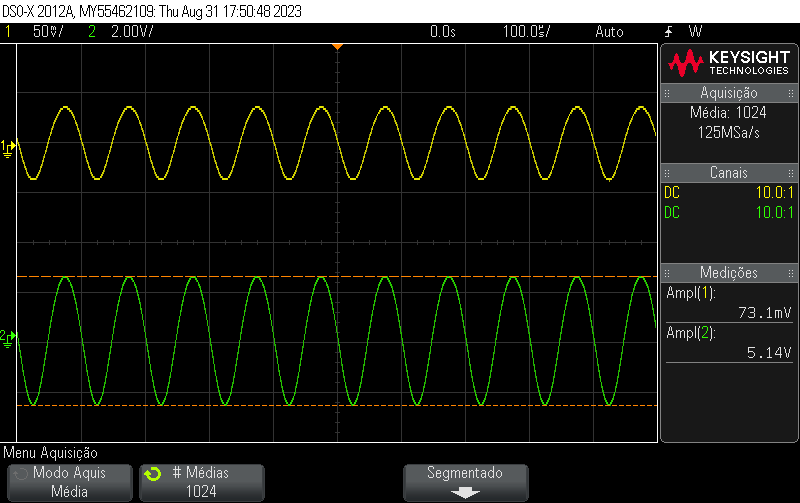
\includegraphics[width=0.5\columnwidth]{images/v_pot1.png}
    \caption{Tensão sobre $R_L$ e o potenciômetro em seu máximo.}
\end{figure}

\begin{figure}[H]
    \centering
    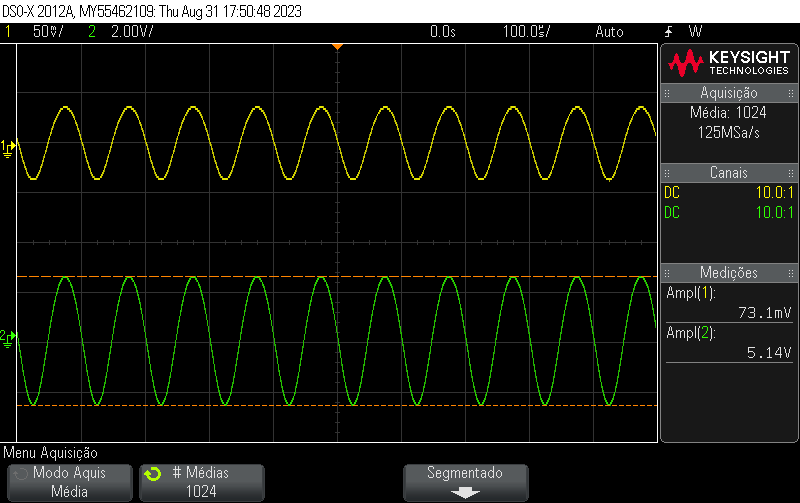
\includegraphics[width=0.5\columnwidth]{images/v_pot1.png}
    \caption{Tensão sobre $R_L$ e o potenciômetro em $75\%$ de seu máximo.}
\end{figure}

\begin{figure}[H]
    \centering
    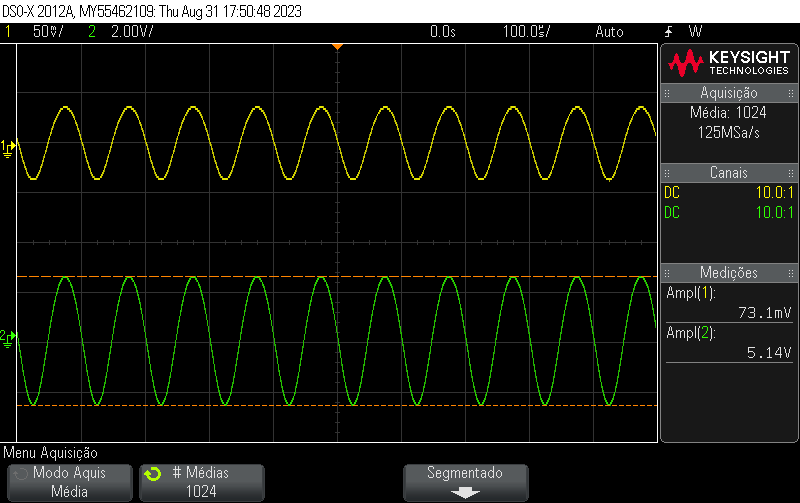
\includegraphics[width=0.5\columnwidth]{images/v_pot1.png}
    \caption{Tensão sobre $R_L$ e o potenciômetro em $50\%$ de seu máximo.}
\end{figure}

\begin{figure}[H]
    \centering
    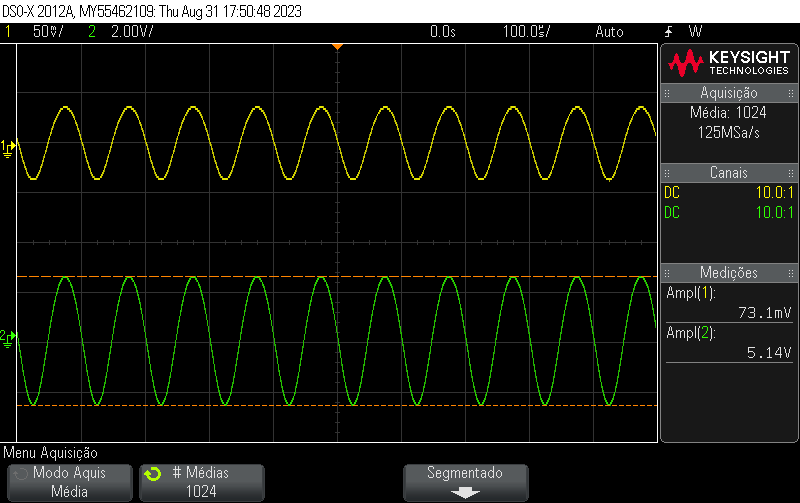
\includegraphics[width=0.5\columnwidth]{images/v_pot1.png}
    \caption{Tensão sobre $R_L$ e o potenciômetro em $25\%$ de seu máximo.}
\end{figure}

\begin{figure}[H]
    \centering
    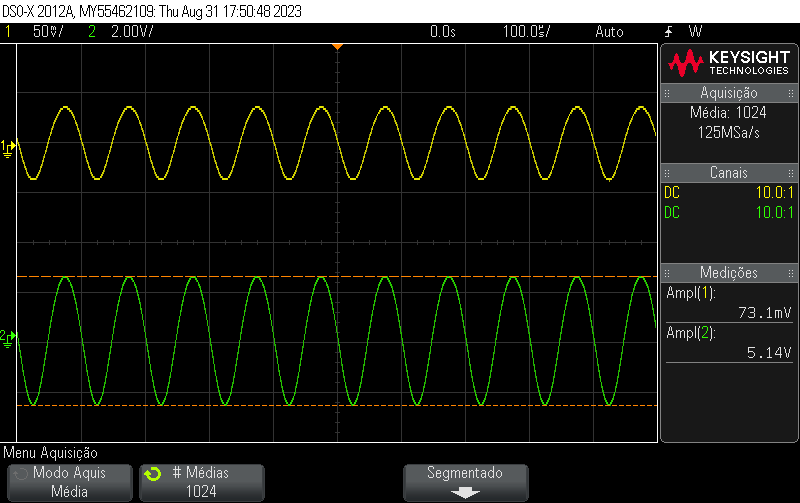
\includegraphics[width=0.5\columnwidth]{images/v_pot1.png}
    \caption{Tensão sobre $R_L$ e o potenciômetro em seu mínimo.}
\end{figure}
